\chapter{Revisão Bibliográfica}
\label{cap:descr}

%% - - - - - - - - - - - - - - - - - - - - - - - - - - - - - - - - - - -
\section{Controle Adaptativo}
\label{sec:adapt}
Sistemas de controle possuem como característica principal a capacidade de interferir no comportamento de outros sistemas, para alcançar um valor desejado. Existe uma subdivisão com base no tipo de método de controle. Temos os controles adaptativos, podendo ser identificados como sendo  aqueles cujo método de controle usado por um determinado controlador se adapta a um sistema controlado por meio de parâmetros que variam ou então que são inicialmente incertos. Åström e Wittenmark \cite{controle_adaptativo_livro} afirmam que o controle adaptativo pode ser entendido como uma metodologia empregada em sistemas de controle que possibilita o ajuste contínuo ao longo do tempo em resposta a mudanças nas condições e ao conhecimento adquirido pelo controlador.

Dentro de controle adaptativo pode-se observar uma macrodivisão, resultando em dois principais tipos de controle adaptativo: feed-forward e Feedback (malha fechada). O esquema de funcionamento geral é ilustrado na Figura \ref{fig:controle_adaptativo}. É importante ressaltar que mesmo com esta macrodivisão uma característica comum é que para estes dois subtipos a base é a estimativa de parâmetros \cite{ac_rl_intersections}.

\begin{figure}[h]
 \centering
%   \subfigure[][Primeira subfigura.]
  \subfigure[][feedforward.]
   {
    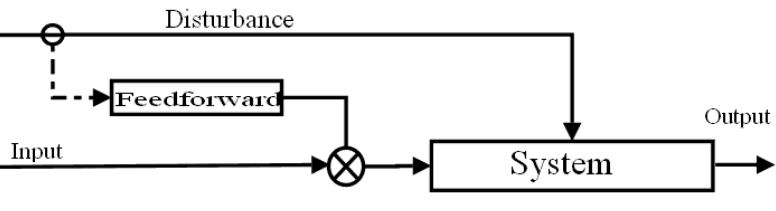
\includegraphics[width=0.45\textwidth]{./fig/feedforward.png}
    \label{subfig:feedforward}
   } \qquad
  \subfigure[feedback.]
   {
    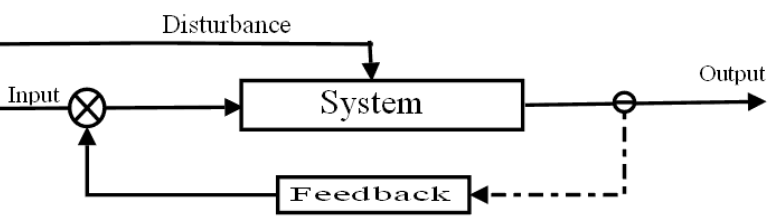
\includegraphics[width=0.45\textwidth]{./fig/feedback.png}
    \label{subfig:feedback}
   }
   \caption{{\subref{subfig:feedforward}} e {\subref{subfig:feedback}} ilustram, respectivamente, sistemas de controle feedforward e feedback.}
  \label{fig:controle_adaptativo}
\end{figure}

Para realizar estimativa de parâmetros são utilizadas algumas técnicas ou estimadores, como a Cadeia de Markov Monte Carlo. Uma cadeia de Markov é uma sequência de eventos, onde a probabilidade de cada evento depende apenas do estado atingido no evento anterior. Matematicamente, uma sequência $X = {X_1, X_2, X_3, ..., X_n}$ de variáveis aleatórias é uma cadeia de Markov se, para qualquer $i$ e qualquer conjunto de estados possíveis $x_1, x_2, ..., x_n$, tem-se a equação \ref{eqn:cadeia_marov}, \cite{introducao_modelos_probabilisticos}. O Método de Monte Carlo é uma técnica estatística que permite a aproximação numérica de quantidades que seriam difíceis ou impossíveis de calcular exatamente. Consiste basicamente em usar a geração de números aleatórios para simular o comportamento de um sistema \cite{monte_carlo_statistical_methods}.

\begin{equation}
    \label{eqn:cadeia_marov}
        P(X_{i+1} = x_{i+1} | X_1 = x_1, X_2 = x_2, \ldots, X_i = x_i) = P(X_{i+1} = x_{i+1} | X_i = x_i)
\end{equation}



%% - - - - - - - - - - - - - - - - - - - - - - - - - - - - - - - - - - -
\section{Aprendizado por Reforço}
\label{sec:RL}
O Aprendizado por Reforço é uma abordagem de Aprendizado de Máquina que lida com o problema de como um agente deve tomar decisões em um ambiente para maximizar recompensa, acumulada ao longo do tempo. Diferente do Aprendizado Supervisionado e do Aprendizado Não Supervisionado, o Aprendizado por Reforço depende principalmente de feedback em forma de recompensas. Estas recompensas são obtidas com base nas interações que o agente realiza no ambiente, que irão guiar a mudança de estado, como ilustra o esquema da Figura \ref{fig:rl_ilustracao}.



\begin{itemize}
\item \textbf{Agente}: O agente é o aprendiz que interage com o ambiente e toma decisões. Ele observa o estado atual do ambiente, escolhe uma ação para executar e recebe feedback na forma de recompensas. 

\item \textbf{Ambiente}: O ambiente é o contexto em que o agente opera e do qual ele obtém informações. Ele é modelado como um sistema no qual o agente pode realizar ações e recebe recompensas com base em suas ações e no estado atual do ambiente. 

\item \textbf{Ações}: As ações representam as decisões que o agente pode tomar em cada etapa de interação com o ambiente. Dependendo do domínio específico, as ações podem ser discretas ou contínuas.


\item \textbf{Recompensas}: As recompensas são os sinais de feedback que o agente recebe do ambiente após cada ação. Elas indicam a qualidade da ação tomada em relação ao objetivo geral do agente. 

\end{itemize}

\begin{figure}[H]
 \centering
 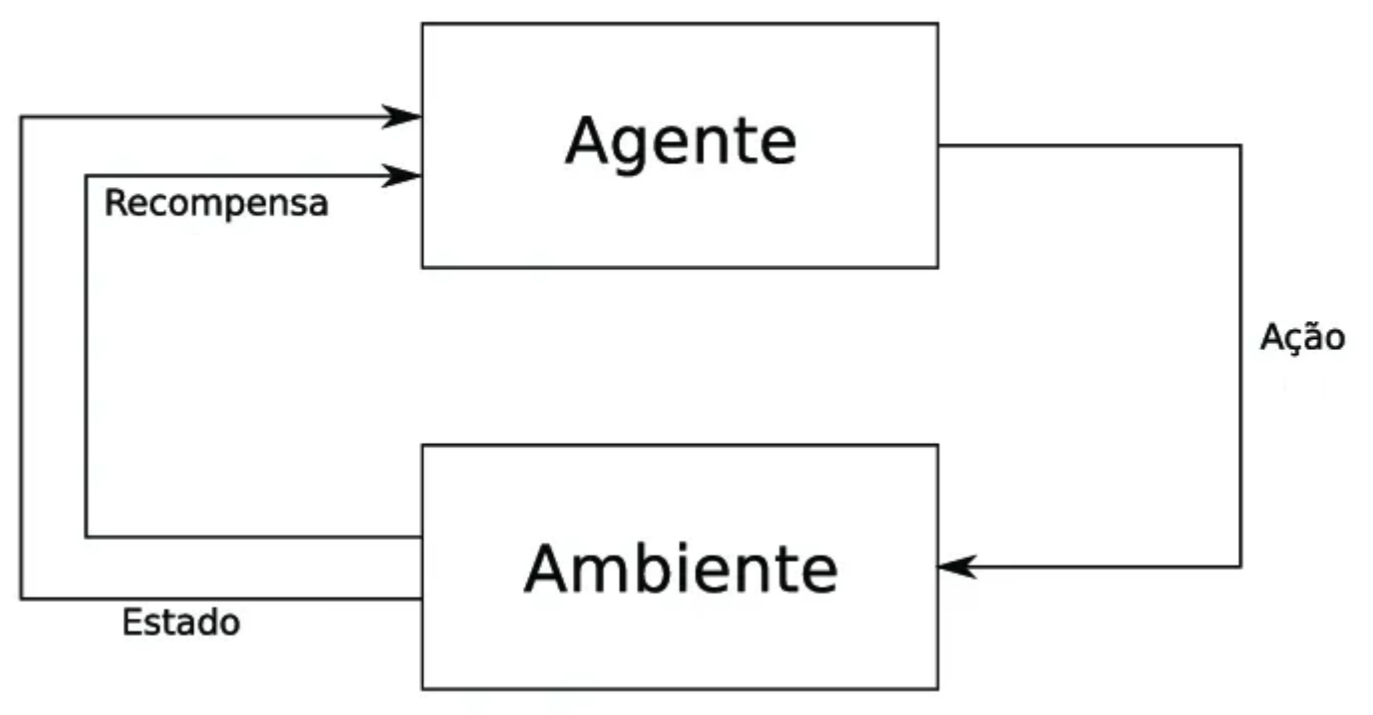
\includegraphics[width=0.60\textwidth]{./fig/RL_ilustracao.png}

 \caption{Ilustração do ciclo de aprendizado.
 Fonte: Wikimedia Commons}
 \label{fig:rl_ilustracao}
\end{figure}

O objetivo do agente é aprender a política que maximize a soma das recompensas ao longo do tempo. Com base em tais características pode-se observar que o agente possui um papel bem definido, sendo que este interage com o ambiente em etapas discretas de tempo, sendo que em cada uma destas etapas o agente executa várias vezes a seguinte sequência de ações:

\begin{enumerate}
\item Observa o estado atual do ambiente.
\item Com base na política aprendida, seleciona uma ação para executar.
\item Executa a ação no ambiente.
\item Recebe uma recompensa do ambiente com base na ação tomada e no estado resultante.
\item Atualiza seu conhecimento e política com base na recompensa recebida.
\end{enumerate}

É possível notar que a lógica de funcionamento do Aprendizado por Reforço é fácil de entender e até mesmo de visualizar \ref{fig:rl_ilustracao}, pois tem muita semelhança com a maneira como os humanos aprendem tarefas novas. Apenas alusões e afirmações vagas não são suficientes para modelar o problema dentro de Aprendizado por reforço, é necessário traduzir toda essa lógica para o contexto computacional. Para isso utiliza-se o modelo matemático chamado Processo de Decisão de Markov (Markov Decision Process - MDP) \cite{sutton}.

\subsection*{Processo de Decisão de Markov - MDP}

Para falar de Processo de Decisão de Markov primeiro é necessário apresentar a Propriedade de Markov. Tal propriedade diz, de forma geral, que uma vez que se tem o presente, o futuro independe do passado \cite{sutton}. De forma mais detalhada, um estado só seguirá a propriedade de Markov caso todos os estados anteriores não tiverem influência na decisão do estado seguinte ao atual.

É fácil entender que nem todos os problemas obedecem a esta propriedade, restringindo o campo de atuação de soluções que utilizem da propriedade de Markov para modelar problemas. Para os contextos onde esta propriedade se aplica a propriedade pode ser descrita pela equação \ref{eqn:propriedade_markov} \cite{sutton}.

\begin{equation}
    \label{eqn:propriedade_markov}
        P\left(S_{t+1} \mid S_t\right)=P\left(S_{t+1} \mid S_1, S_2, \ldots, S_t\right)
\end{equation}

\begin{itemize}
\item  \textbf{$P(S_{t+1} \mid S_t)$}: Probabilidade de acontecimento do estado $S_{t+1}$, dado que o estado $S_{t}$ ocorreu.
\item  \textbf{ $S_{t}$}: Estado atual.
\item  \textbf{ $S_{t+1}$}: Estado seguinte.
\item  \textbf{ $P(S_{t+1} \mid S_1, S_2, \ldots, S_t)$ }: Probabilidade de ocorrer o estado $S_{t+1}$, dado que qualquer um dos estados  $(S_1, S_2, \ldots, S_t)$ aconteça.
\end{itemize}


O entendimento direto desta equação é que a probabilidade de acontecer o estado  $S_{t+1}$, estando no estado  $S_t$, é igual à probabilidade de o estado  $S_{t+1}$ acontecer, estando em qualquer um dos estados$(S_1, S_2, \ldots, S_t)$. Ou seja, todos os estados antes do atual não possuem relevância para o acontecimento do estado novo, no caso,  $S_{t+1}$.

Partindo da propriedade de Markov, agora possui-se contexto para entender o funcionamento do MDP. É através do MDP que se obtém o ferramental matemático para modelar o processo de tomada de decisão em contextos onde os resultados são em parte aleatórios e em parte sob o controle de um tomador de decisão \cite{sutton}. Na Figura \ref{fig:MDP} é apresentada a formalização das nomenclaturas supracitadas, que compõe o processo de interação do agente no ambiente, em MDP. De forma geral, o agente utiliza as informações fornecidas pelo MDP para aprender a melhor política de ação, levando em consideração o estado atual e as recompensas esperadas a longo prazo, como ilustrado na Figura \ref{fig:MDP}.

\begin{figure}[H]
 \centering
 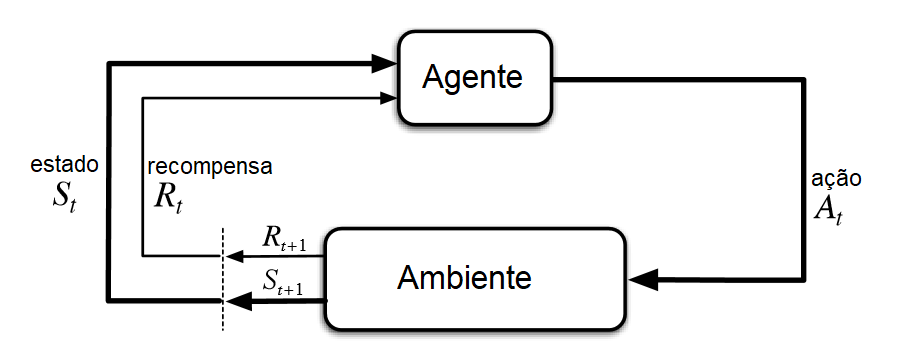
\includegraphics[width=0.65\textwidth]{./fig/MDP.png}

 \caption{Interação agente-ambiente em um Processo de Decisão
de Markov \cite{sutton}.}
 \label{fig:MDP}
\end{figure}


Agora, já formalizado o MDP, o ciclo de tomada de decisão fica sendo o seguinte:

\begin{enumerate}
\item O agente está em um determinado estado $(S_t)$ no ambiente.
\item Com base na política aprendida, seleciona uma ação $(A_t)$ para executar.
\item Executa a ação no ambiente $P(S_{t+1} \mid S_1, S_2, \ldots, S_t)$.
\item Recebe uma recompensa $(R_t)$ do ambiente com base na ação tomada  $(A_t)$ e o estado resultante $(S_{t+1})$.
\item Atualiza seu conhecimento e política com base na recompensa recebida.
\end{enumerate}

Essa sequência representa uma interação e uma sequência de interações entre o agente e o ambiente, recebe o nome de episódio. Com isso, em um episódio o agente toma várias ações e, consequentemente, recebe as respectivas recompensas. Como cada problema possui sua particularidade, tem-se que a duração destes episódios pode variar conforme o tipo de problema que está sendo abordado.
%% - - - - - - - - - - - - - - - - - - - - - - - - - - - - - - - - - - -
\section{Algoritmo Dreamer}
\label{sec:dreamer}
O Dreamer surgiu como proposta para desenvolver um agente de RL que aprende comportamentos de longo prazo puramente por meio de imaginação latente. Para isso, são utilizados modelos de mundo, aprendidos para resumir a experiência de um agente e facilitar a aprendizagem de comportamentos complexos. Esses modelos de mundo são capazes de fazer previsões sobre o futuro com base em observações passadas. No caso do Dreamer, as previsões são feitas em um espaço latente compacto, o que permite uma aprendizagem eficiente de comportamentos ao propagar gradientes analíticos dos valores de estado aprendidos por meio de trajetórias imaginadas. Além disso, otimiza uma política paramétrica por meio da propagação de gradientes analíticos de valores de vários passos através das dinâmicas latentes aprendidas \cite{dream_v1}.

A arquitetura do algoritmo Dreamer consiste em três componentes principais Figura \ref{fig:componentes_dreamer}:  \textbf{aprendizado de dinâmicas latentes, aprendizado de comportamento e interação com o ambiente}.
\begin{itemize}
\item \textbf{Aprendizado de dinâmicas latentes}: o agente aprende um modelo de mundo a partir de experiências passadas, que consiste em um modelo de representação, um modelo de transição e um modelo de recompensa. O modelo de representação codifica observações e ações em estados latentes compactos, o modelo de transição prevê os estados futuros com base nos estados anteriores e ações, e o modelo de recompensa prevê as recompensas com base nos estados.
\item \textbf{Aprendizado de comportamento}:  o agente aprende a selecionar ações e estimar valores de estado com base nas trajetórias imaginadas no espaço latente. É aqui onde o agente utiliza gradientes analíticos dos valores de estado para otimizar a política.
\item \textbf{ Interação com o ambiente}: o agente executa a política aprendida no mundo real para coletar novas experiências e expandir o conjunto de dados.
\end{itemize}

\subsection*{Aprendizado por Reforço e o algoritmo Dreamer}
O Aprendizado por Reforço é incorporado no algoritmo Dreamer no mecanismo de aprendizagem do modelo de valor. Este modelo estima as recompensas imaginadas que o modelo de ação alcança a partir de cada estado. Isso permite que o agente aprenda a maximizar as recompensas imaginadas além do horizonte de imaginação \cite{dream_v1}, as chamadas tarefas de longo horizonte (long-horizon).

\begin{figure}[h]
 \centering
%   \subfigure[][Primeira subfigura.]
  \subfigure[][Aprende a dinâmica latente com a experiência.]
   {
    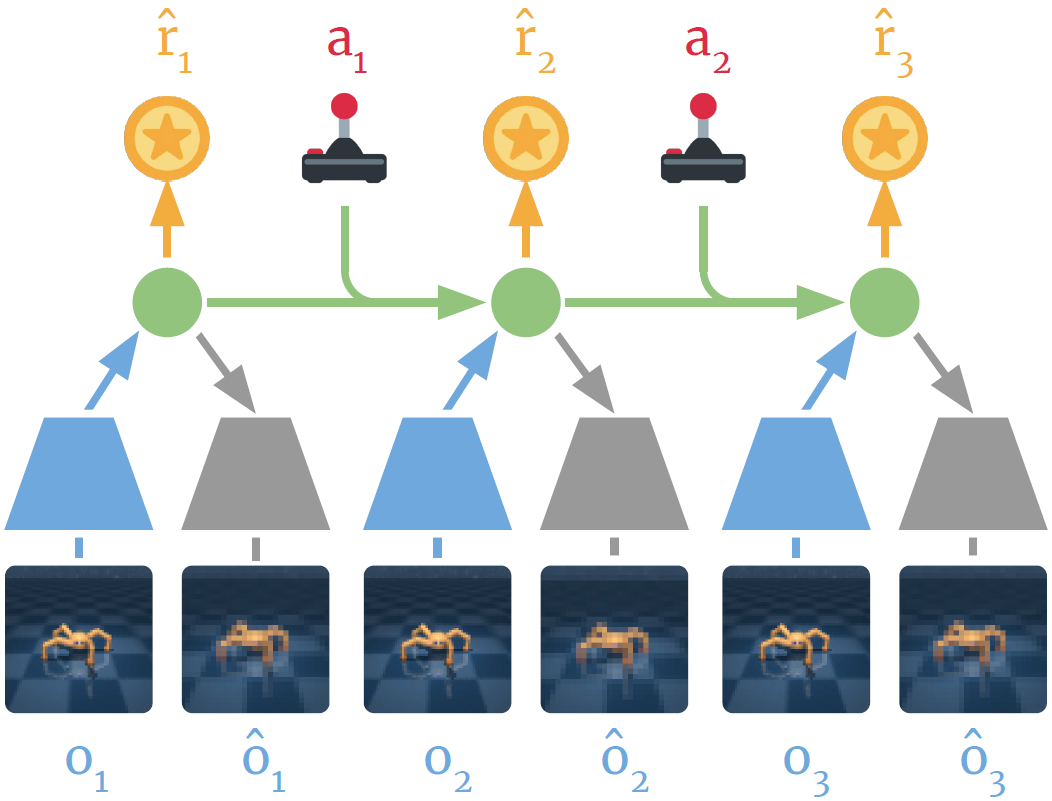
\includegraphics[width=0.25\textwidth]{./fig/componentes_dreamer_a.png}
    \label{subfig:aprende_dinamica}
   } \qquad
  \subfigure[Aprende o comportamento na imaginação.]
   {
    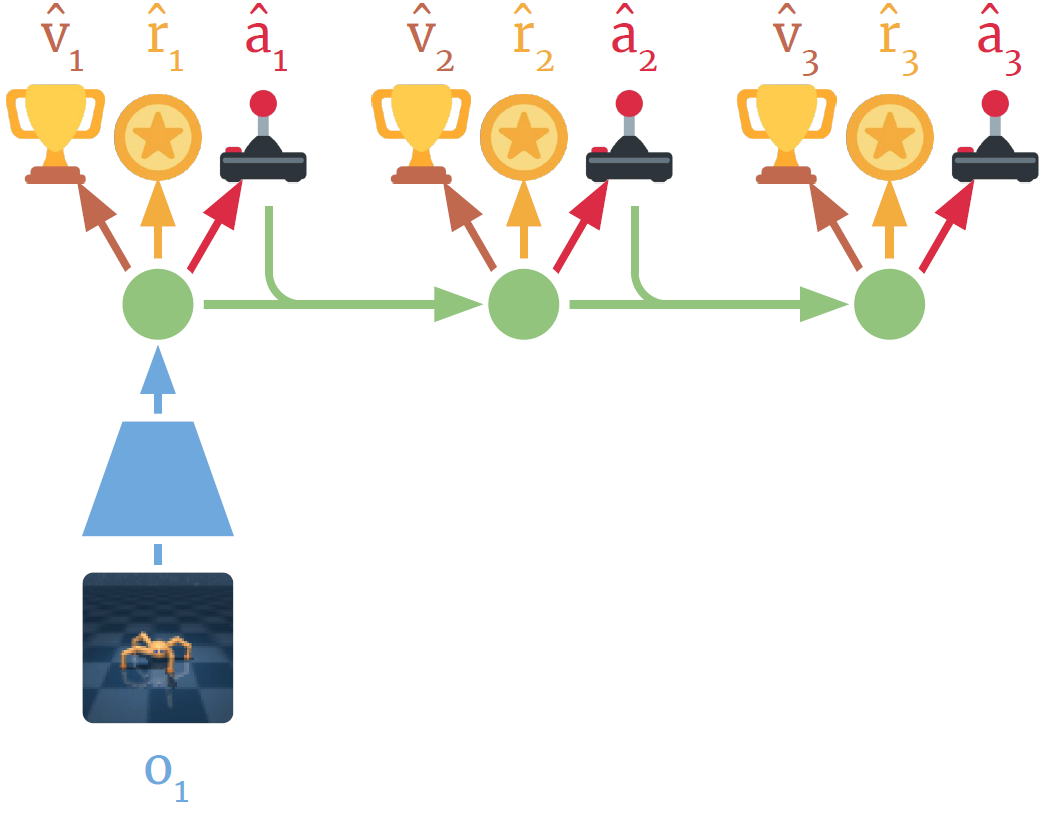
\includegraphics[width=0.25\textwidth]{./fig/componentes_dreamer_b.png}
    \label{subfig:aprende_comportamento}
   }\qquad
  \subfigure[Interage no ambiente.]
   {
    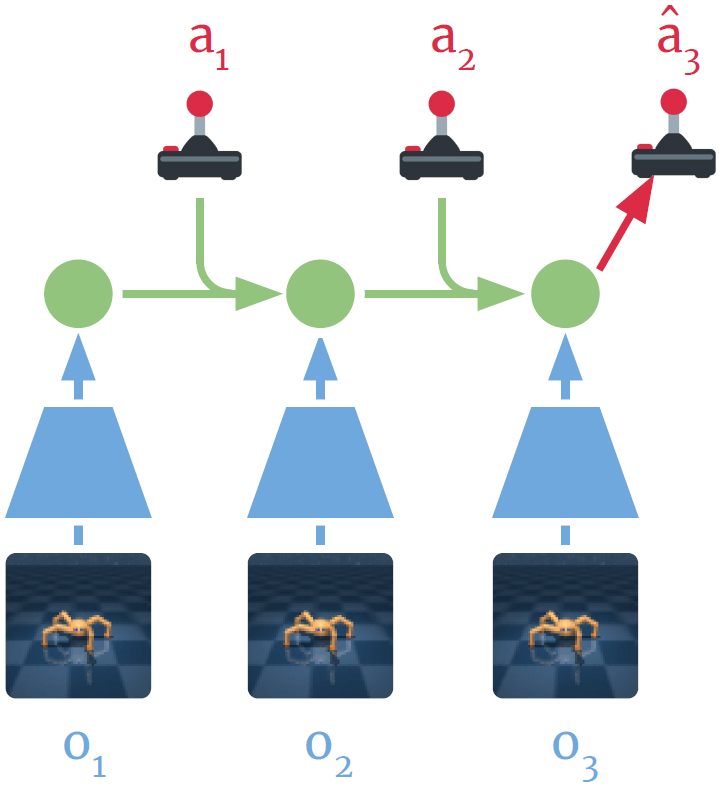
\includegraphics[width=0.25\textwidth]{./fig/componentes_dreamer_c.png}
    \label{subfig:age_ambiente}
   }
   \caption{Componentes do Dreamer. {\subref{subfig:aprende_dinamica}} A partir do dataset de experiência passada, o agente aprende a codificar observações e ações em estados latentes compactos, por exemplo, por meio de reconstrução, e prevê recompensas do ambiente.
    {\subref{subfig:aprende_comportamento}} No espaço latente compacto, o Dreamer prevê valores de estado e ações que maximizam as previsões de valor futuro, propagando gradientes de volta por meio de trajetórias imaginadas.
    {\subref{subfig:age_ambiente}} O agente codifica o histórico do episódio para calcular o estado atual do modelo e prever a próxima ação a ser executada no ambiente \cite{dream_v1}.}
  \label{fig:componentes_dreamer}
\end{figure}

Neste sentido,  o Dreamer utiliza uma abordagem de ator-crítico \textbf{(actor-critic)} para aprender comportamentos que consideram recompensas além do horizonte de imaginação. O Dreamer aprende um modelo de ação e um modelo de valor no espaço latente do modelo do mundo. O modelo de ação implementa a política e visa prever ações que resolvam o ambiente de imaginação. O modelo de valor estima as recompensas imaginadas esperadas que o modelo de ação alcança a partir de cada estado. Ambos os modelos são treinados cooperativamente, onde o modelo de ação visa maximizar uma estimativa do valor, enquanto o modelo de valor visa corresponder a uma estimativa do valor que muda à medida que o modelo de ação muda. O modelo de valor é atualizado para se ajustar aos alvos de valor estimados, enquanto o modelo de ação usa gradientes analíticos através das dinâmicas aprendidas para maximizar as estimativas de valor.

Como as previsões são usadas para tomar decisões sobre as ações a serem executadas pelo agente no ambiente. O processo parcialmente observável de decisão de Markov \textbf{(partially observable Markov decision
process - POMDP)} é usado para modelar a interação entre o agente e o ambiente, permitindo que o agente tome decisões com base nas informações disponíveis no estado atual e nas ações possíveis \cite{dream_v1}.


%Com isso a sequencia de passos e a organização de cada parte do algoritmo pode ser representada no pseudo algoritmo [PSEUDO ALGORITMO DO DREAMER]


\section{Futebol de Robôs}
O futebol de robôs é um campo de pesquisa interdisciplinar combinando conhecimentos de várias áreas como Robótica, Controle e Inteligência Artificial para desenvolver sistemas autônomos que sejam capazes de jogar futebol, se comportando como um time. Cada robô é um agente autônomo, tomando decisões independentes e cooperando para alcançar o objetivo da equipe, no caso, ganhar a partida (fazendo o maior número de gols na partida).

Dentro do contexto de futebol de robôs existem várias categorias que possuem o mesmo objetivo, fazer robôs autônomos que jogam futebol). Um exemplo disso é a Competição Brasileira de Robótica - CBR \cite{cbr_site} que reúne categorias como Humanoid League (futebol com humanoides), Small Size Soccer (futebol com robôs pequenos) e Very Small Size Soccer - VSSS (futebol com robôs bem pequenos, mais simples). Este trabalho aborda a categoria VSSS, por ser mais simples e por já existirem modelagens do ambiente, que facilitam nas simulações, quando necessário.

Os desafios presentes no VSSS já foram abordados com propostas de soluções que utilizam de RL \cite{bruno_brandao}, \cite{robocin} como plano de fundo. com isso, e sabendo das intersecções entre controle adaptativo e RL \cite{ac_rl_intersections}, entende-se mais sobre o contexto do futebol de robôs, mais especificamente do VSSS.


\subsection*{Categoria Very Small Size Soccer - VSSS }

A categoria Very Small Size Soccer (VSSS) pertence à competição de futebol de robôs, onde duas equipes de três robôs cada competem para marcar gols no time oponente. Os robôs possuem apenas duas rodas e devem ser autônomos durante a partida, utilizando estratégias de controle e tomada de decisão para jogar.

Algumas das principais características da categoria são:

\begin{itemize}
    \item \textbf{Campo e bola}: O campo é composto por uma chapa plana de madeira, com marcações específicas, e a bola utilizada é laranja, com aproximadamente 42.7mm de diâmetro e 46g de massa.
    
    \item \textbf{Jogadores}: Cada time é composto por no máximo 3 robôs, sendo permitido apenas um goleiro. Durante o jogo, apenas 3 membros de cada time podem estar no campo.
    
    \item \textbf{Regras de jogo}: Existem regras específicas para o início do jogo, substituições, interrupções durante o jogo, tiro livre, pênalti, entre outras situações \cite{regras_vss2023}.
    
    \item \textbf{Sistema de visão}: É permitido o uso de um sistema de visão, por equipe, para identificar os robôs e a bola em campo.
    
    \item \textbf{Duração do jogo}: Cada partida tem dois períodos de 5 minutos, com um intervalo de meio tempo de 10 minutos.
    
    \item \textbf{Método de pontuação}: Os gols são computados quando a bola passa inteiramente por cima da linha do gol. O vencedor é determinado pelo número de gols marcados.
\end{itemize}


O ambiente onde acontecem os jogos é representado na Figura \ref{fig:ambiente_vsss}, mas pode ser resumido na seguinte sequência de passos, sendo executada repetidamente até que o jogo pare:

\begin{itemize}
    \item \textbf{Câmera:} captura a imagem da visão superior do campo e envia para os respectivos servidores (computadores)
    
    \item \textbf{Servidor:} extrai informações a partir das imagens (orientações e posição)
    
    \item \textbf{Servidor:} Calcula qual a próxima ação e define os alvos
    
    \item \textbf{Servidor:} envia os comandos de velocidades para os respectivos robôs

    \item \textbf{Robôs:} executam os comandos recebidos
\end{itemize}


    \begin{figure}[H]
     \centering
     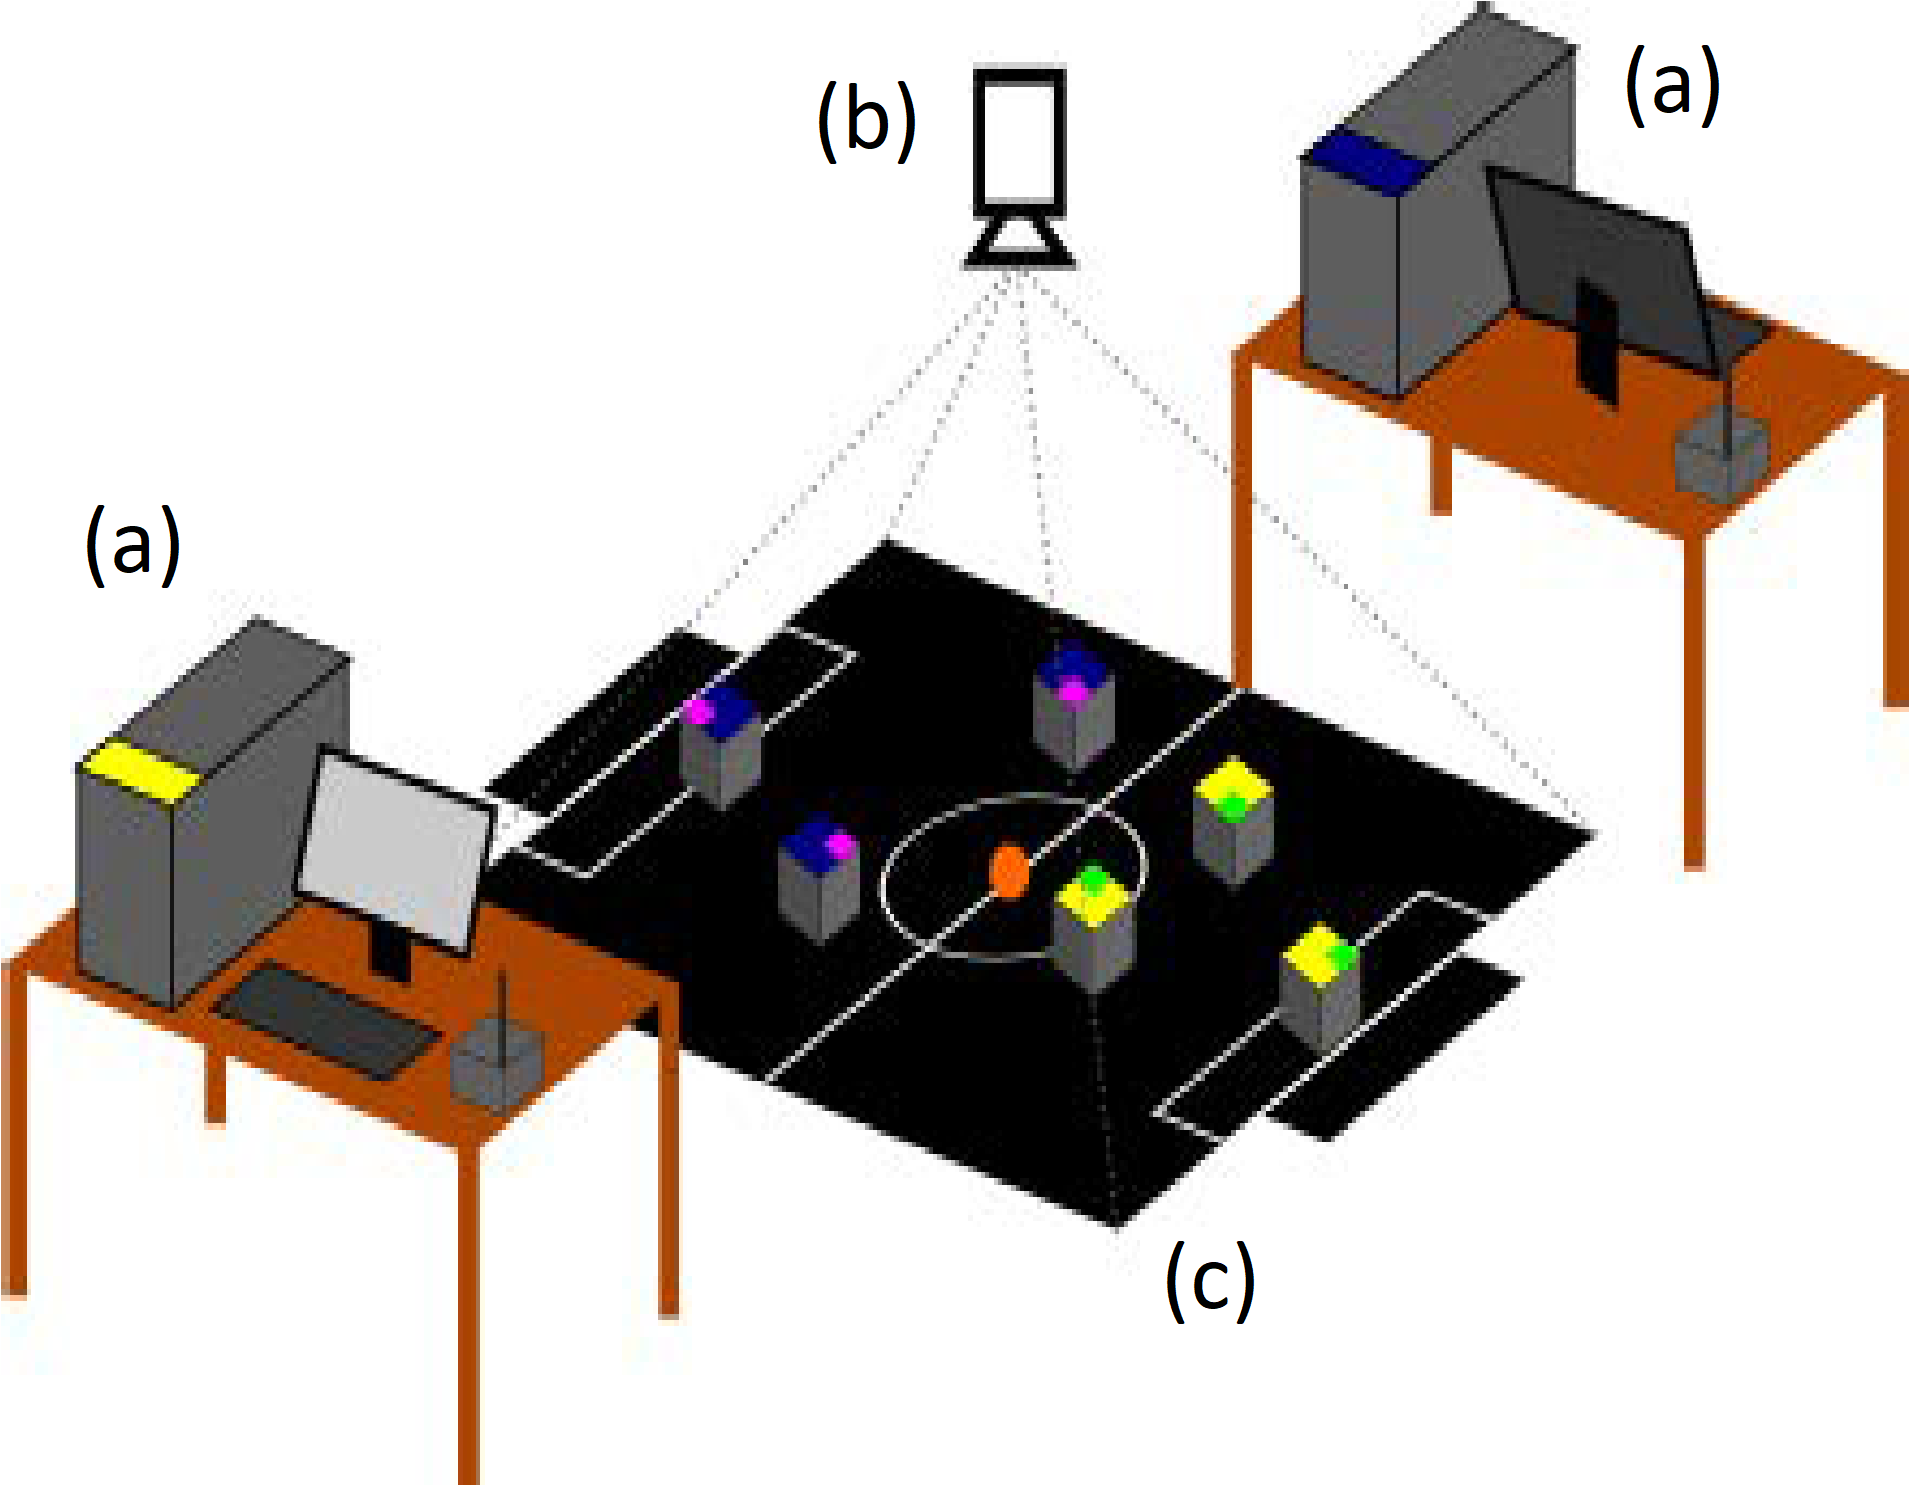
\includegraphics[width=0.50\textwidth]{./fig/ambiente_vsss.png}
    
     \caption{Ambiente de uma partida da categoria Very Small Size Soccer. (a) São os servidores de cada equipe. (b) Câmera que capta as imagens do jogo e envia para os respectivos servidores, sempre vista superior. (c) Campo onde acontecem as jogadas dos robôs, que recebem comandos dos servidores}
     \label{fig:ambiente_vsss}
    \end{figure}

    
